\documentclass[tikz,border=6pt,11pt]{standalone}
\usepackage{amsmath,amssymb}
\usepackage{xcolor}
\definecolor{accent}{HTML}{A13D2C}
\definecolor{accent2}{HTML}{2B5F6B}
\definecolor{muted}{HTML}{5A564F}
\definecolor{panel}{HTML}{F8F6F0}
\definecolor{linecol}{HTML}{D8D2C4}
\definecolor{astroblue}{HTML}{1B4F72}
\definecolor{ink}{HTML}{1E1C1A}
\usetikzlibrary{calc}
\usepackage[T1]{fontenc}\usepackage{newpxtext,newpxmath}  % same fonts as the notes
\begin{document}
% Zoom ladder, schematic, 15.4 cm wide (the text width) so the type is its true size. Reading order 1 to 5 snakes
% along the top row and back along the bottom row. Each box is 4.7 cm square. Its sketch area is the part above the
% label strip. All sketches are drawn from formulas, with no random numbers (golden-angle sequences instead).
% Box widths shown, for the scale bars: galaxy 130 kpc, group 4 Mpc, cluster 8 Mpc, supercluster 250 Mpc, web 1 Gpc.
% The red square in a box marks the previous box, and the grey lines run from the corners of that box.
\newcommand{\dotsalong}[7]{% x1 y1 x2 y2 count jitter radius: dots along a segment, crowded toward both ends (the nodes)
  \pgfmathsetmacro{\segL}{veclen((#3)-(#1),(#4)-(#2))}
  \foreach \k in {1,...,#5} {
    \pgfmathsetmacro{\t}{0.5-0.5*cos(180*(\k-0.5+0.3*sin(\k*211))/(#5))}
    \pgfmathsetmacro{\j}{(#6)*sin(\k*137.5+(#1)*57+(#2)*31)}
    \fill[ink] ({(#1)+\t*((#3)-(#1))-\j*((#4)-(#2))/\segL},{(#2)+\t*((#4)-(#2))+\j*((#3)-(#1))/\segL}) circle[radius=#7];
  }}
\newcommand{\ball}[5]{% x y R count radius: a round clump of dots that thickens to the centre
  \foreach \k in {1,...,#4} {
    \pgfmathsetmacro{\r}{(#3)*exp(1.6*ln((\k-0.5)/(#4)))}
    \fill[ink] ({(#1)+\r*cos(\k*137.508)},{(#2)+\r*sin(\k*137.508)}) circle[radius=#5];
  }}
\newcommand{\spiral}[6]{% x y scale rotation flattening dotradius: two-armed log spiral r = 0.1 exp(0.3 t), t = 0 .. 7.68
  \begin{scope}[shift={(#1,#2)}, rotate=#4, scale=#3, yscale=#5]
    \shade[inner color=accent!55!white, outer color=panel] (0,0) circle[radius=0.3];
    \foreach \s in {0,180} {
      \draw[astroblue!70, line width=1.1pt] plot[domain=0:7.68, samples=70, smooth] ({0.1*exp(0.3*\x)*cos(\x r+\s)}, {0.1*exp(0.3*\x)*sin(\x r+\s)});
    }
    \ifdim #6 pt>0pt
    \foreach \s in {0,180} {
      \foreach \k in {1,...,110} {
        \pgfmathsetmacro{\th}{7.68*(\k-0.5)/110}
        \pgfmathsetmacro{\rr}{0.1*exp(0.3*\th)*(1+0.12*sin(\k*131))}
        \pgfmathsetmacro{\aa}{deg(\th)+\s+9*sin(\k*77)}
        \fill[astroblue] ({\rr*cos(\aa)},{\rr*sin(\aa)}) circle[radius=#6/#3];
      }
    }
    \fi
  \end{scope}}
\newcommand{\ellip}[6]{% x y rx ry angle colour: a smooth oval galaxy
  \fill[#6, rotate around={#5:(#1,#2)}] (#1,#2) ellipse[x radius=#3, y radius=#4];}
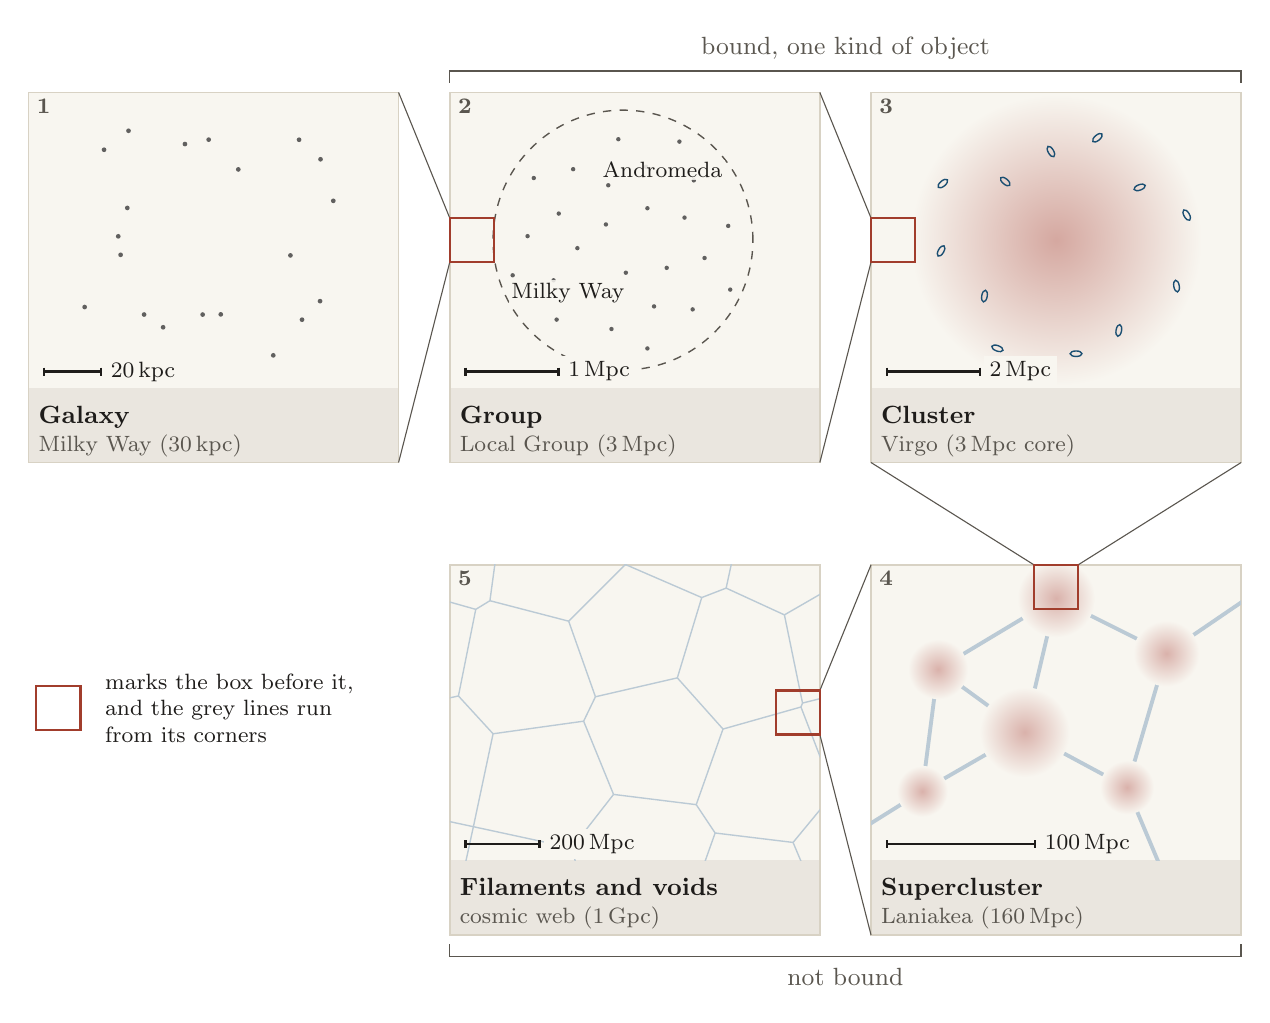
\begin{tikzpicture}[x=1cm,y=1cm, font=\small]
  \def\S{4.7}\def\hb{2.35}\def\ys{0.475}% box side, half side, height of the sketch centre above the box centre
  \def\sh{1.875}% half height of the sketch area
  % box centres (cx,cy): 1 galaxy, 2 group, 3 cluster along the top, 4 supercluster below the cluster, 5 web to its left
  \def\cxa{0}  \def\cya{0}
  \def\cxb{5.35}\def\cyb{0}
  \def\cxc{10.7}\def\cyc{0}
  \def\cxd{10.7}\def\cyd{-6.0}
  \def\cxe{5.35}\def\cye{-6.0}
  % boxes with label strips
  \foreach \cx/\cy/\num/\name/\detail in {
      \cxa/\cya/1/Galaxy/Milky Way (30\,kpc),
      \cxb/\cyb/2/Group/Local Group (3\,Mpc),
      \cxc/\cyc/3/Cluster/Virgo (3\,Mpc core),
      \cxd/\cyd/4/Supercluster/Laniakea (160\,Mpc),
      \cxe/\cye/5/Filaments and voids/cosmic web (1\,Gpc)} {
    \fill[panel] (\cx-\hb,\cy-\hb) rectangle (\cx+\hb,\cy+\hb);
    \fill[linecol!55] (\cx-\hb,\cy-\hb) rectangle (\cx+\hb,\cy-\hb+0.95);
    \draw[linecol, line width=0.6pt] (\cx-\hb,\cy-\hb) rectangle (\cx+\hb,\cy+\hb);
    \node[ink, anchor=base west, inner sep=0] at (\cx-\hb+0.12,\cy-\hb+0.5) {\textbf{\name}};
    \node[muted, font=\footnotesize, anchor=base west, inner sep=0] at (\cx-\hb+0.12,\cy-\hb+0.14) {\detail};
    \node[muted, font=\footnotesize\bfseries, anchor=north west, inner sep=0] at (\cx-\hb+0.1,\cy+\hb-0.08) {\num};
  }
  % ---------- 1 Milky Way with the two Magellanic Clouds
  \begin{scope}[shift={(\cxa,\cya+\ys)}]
    \clip (-\hb,-\sh) rectangle (\hb,\sh);
    \spiral{0}{0}{0.95}{25}{0.8}{0.026}
    \ellip{1.5}{1.0}{0.17}{0.11}{30}{accent2}   % Large Magellanic Cloud, 50 kpc away
    \ellip{1.95}{0.3}{0.1}{0.07}{10}{accent2}   % Small Magellanic Cloud, 60 kpc away
    \foreach \k in {1,...,20} {                % dwarf spheroidals
      \pgfmathsetmacro{\r}{1.0+0.9*sin(\k*83)*sin(\k*83)}
      \fill[ink!70] ({\r*cos(\k*137.5)},{0.9*\r*sin(\k*137.5)}) circle[radius=0.03];
    }
    \draw[ink, line width=0.8pt] (-2.15,-1.67) -- ++(0.72,0) (-2.15,-1.62) -- ++(0,-0.1) (-1.43,-1.62) -- ++(0,-0.1);
    \node[ink, font=\footnotesize, anchor=west, inner sep=2pt, fill=panel] at (-1.38,-1.67) {20\,kpc};
  \end{scope}
  % ---------- 2 Local Group, two big spirals and a scatter of dwarfs
  \begin{scope}[shift={(\cxb,\cyb+\ys)}]
    \clip (-\hb,-\sh) rectangle (\hb,\sh);
    \draw[muted, dashed, line width=0.5pt] (-0.15,0) circle[radius=1.65];
    \foreach \k in {1,...,26} {
      \pgfmathsetmacro{\r}{1.5*sqrt(\k/26)}
      \fill[ink!70] ({-0.15+\r*cos(\k*137.508)},{\r*sin(\k*137.508)}) circle[radius=0.028];
    }
    \spiral{-0.85}{-0.1}{0.36}{20}{0.8}{0}      % Milky Way
    \spiral{0.55}{0.35}{0.44}{-60}{0.4}{0}      % Andromeda, tilted
    \spiral{0.3}{-0.8}{0.16}{70}{0.7}{0}        % Triangulum
    \node[ink, font=\footnotesize, anchor=north, inner sep=1pt, fill=panel, fill opacity=0.85, text opacity=1] at (-0.85,-0.5) {Milky Way};
    \node[ink, font=\footnotesize, anchor=south, inner sep=1pt, fill=panel, fill opacity=0.85, text opacity=1] at (0.35,0.75) {Andromeda};
    \draw[ink, line width=0.8pt] (-2.15,-1.67) -- ++(1.18,0) (-2.15,-1.62) -- ++(0,-0.1) (-0.97,-1.62) -- ++(0,-0.1);
    \node[ink, font=\footnotesize, anchor=west, inner sep=2pt, fill=panel] at (-0.92,-1.67) {1\,Mpc};
  \end{scope}
  % ---------- 3 Cluster, mostly ellipticals, thickening to the centre, hot gas glow
  \begin{scope}[shift={(\cxc,\cyc+\ys)}]
    \clip (-\hb,-\sh) rectangle (\hb,\sh);
    \shade[inner color=accent!45, outer color=panel] (0,0) circle[radius=1.85];
    \foreach \k in {1,...,120} {
      \pgfmathsetmacro{\r}{1.7*exp(1.7*ln((\k-0.5)/120))}
      \pgfmathsetmacro{\ga}{mod(mod(\k,60)*137.508+int(\k/60)*90.48,360)}
      \pgfmathsetmacro{\px}{\r*cos(\ga)}
      \pgfmathsetmacro{\py}{0.9*\r*sin(\ga)}
      \pgfmathsetmacro{\rx}{0.035+0.03*abs(sin(\k*47))}
      \pgfmathsetmacro{\ry}{\rx*(0.5+0.4*abs(cos(\k*29)))}
      \pgfmathsetmacro{\ang}{mod(\k*61,180)}
      \ellip{\px}{\py}{\rx}{\ry}{\ang}{ink!75}
    }
    \ellip{0}{0}{0.14}{0.1}{20}{ink}
    \foreach \k in {1,...,12} {                    % a few spirals in the outskirts
      \pgfmathsetmacro{\r}{1.0+0.7*abs(sin(\k*67))}
      \pgfmathsetmacro{\qx}{\r*cos(\k*151)}
      \pgfmathsetmacro{\qy}{0.9*\r*sin(\k*151)}
      \pgfmathsetmacro{\ang}{mod(\k*40,180)}
      \draw[astroblue, line width=0.5pt, rotate around={\ang:(\qx,\qy)}] (\qx,\qy) ellipse[x radius=0.075, y radius=0.035];
    }
    \draw[ink, line width=0.8pt] (-2.15,-1.67) -- ++(1.18,0) (-2.15,-1.62) -- ++(0,-0.1) (-0.97,-1.62) -- ++(0,-0.1);
    \node[ink, font=\footnotesize, anchor=west, inner sep=2pt, fill=panel] at (-0.92,-1.67) {2\,Mpc};
  \end{scope}
  % ---------- 4 Supercluster, clusters joined by filaments
  \begin{scope}[shift={(\cxd,\cyd+\ys)}]
    \clip (-\hb,-\sh) rectangle (\hb,\sh);
    \foreach \ax/\ay/\bx/\by in {0/1.45/-1.5/0.55, 0/1.45/1.4/0.75, 0/1.45/-0.4/-0.25, -1.5/0.55/-0.4/-0.25, -1.5/0.55/-1.7/-1.0,
        -0.4/-0.25/0.9/-0.95, 1.4/0.75/0.9/-0.95, -0.4/-0.25/-1.7/-1.0, 1.4/0.75/2.5/1.5, -1.7/-1.0/-2.5/-1.5, 0.9/-0.95/1.3/-1.9} {
      \draw[astroblue!30, line width=1.4pt] (\ax,\ay) -- (\bx,\by);
      \pgfmathtruncatemacro{\N}{max(2,round(veclen(\bx-\ax,\by-\ay)*10))}
      \dotsalong{\ax}{\ay}{\bx}{\by}{\N}{0.05}{0.02}
    }
    \foreach \x/\y/\R/\N in {0/1.45/0.26/40, -1.5/0.55/0.2/30, 1.4/0.75/0.22/34, -0.4/-0.25/0.3/46, 0.9/-0.95/0.18/26, -1.7/-1.0/0.17/24} {
      \shade[inner color=accent!40, outer color=panel] (\x,\y) circle[radius={1.9*\R}];
      \ball{\x}{\y}{\R}{\N}{0.026}
    }
    \draw[ink, line width=0.8pt] (-2.15,-1.67) -- ++(1.88,0) (-2.15,-1.62) -- ++(0,-0.1) (-0.27,-1.62) -- ++(0,-0.1);
    \node[ink, font=\footnotesize, anchor=west, inner sep=2pt, fill=panel] at (-0.22,-1.67) {100\,Mpc};
  \end{scope}
  % ---------- 5 Cosmic web, a foam of empty cells
  % Cell walls are the Voronoi edges of these 20 seed points (x,y in cm from the sketch centre), cut at |x|=3.4, |y|=2.6.
  % Each edge lies on the bisector of two seeds and is cut where a third seed becomes nearer.
  %   (-2.9,-2.0) (-1.5,-2.3) (0.1,-1.9) (1.5,-2.4) (2.9,-1.8) (-2.6,-0.6) (-1.2,-0.9) (0.3,-0.3) (1.7,-0.8) (3.0,-0.3)
  %   (-2.9,0.8) (-1.4,0.5) (0.0,1.0) (1.3,0.6) (2.7,0.9) (-2.5,2.2) (-1.0,2.0) (0.6,2.4) (2.0,2.1) (3.2,2.3)
  % Galaxies sit along the walls and crowd toward the nodes where walls meet. The cells inside stay empty.
  \begin{scope}[shift={(\cxe,\cye+\ys)}]
    \clip (-\hb,-\sh) rectangle (\hb,\sh);
    \foreach \ax/\ay/\bx/\by in {-2.30/-2.60/-2.05/-1.45,-2.05/-1.45/-3.40/-1.16,-0.57/-2.60/-0.80/-1.72,-0.80/-1.72/-2.05/-1.45,0.64/-2.60/1.02/-1.53,-0.27/-1.04/-0.80/-1.72,0.78/-1.17/-0.27/-1.04,1.02/-1.53/0.78/-1.17,2.41/-2.60/2.01/-1.65,2.01/-1.65/1.02/-1.53,2.53/-1.02/2.01/-1.65,3.40/-1.08/2.53/-1.02,-2.05/-1.45/-1.80/-0.27,-2.24/0.21/-3.40/-0.04,-1.80/-0.27/-2.24/0.21,-0.27/-1.04/-0.65/-0.11,-0.65/-0.11/-1.80/-0.27,0.78/-1.17/1.12/-0.21,-0.50/0.20/-0.65/-0.11,0.54/0.44/-0.50/0.20,1.12/-0.21/0.54/0.44,2.53/-1.02/2.11/0.07,2.11/0.07/1.12/-0.21,2.13/0.12/2.11/0.07,3.40/0.44/2.13/0.12,-2.24/0.21/-2.02/1.31,-2.02/1.31/-3.40/1.70,-0.50/0.20/-0.84/1.16,-1.84/1.42/-2.02/1.31,-0.84/1.16/-1.84/1.42,0.54/0.44/0.85/1.46,-0.12/1.88/-0.84/1.16,0.85/1.46/-0.12/1.88,2.13/0.12/1.90/1.24,1.16/1.58/0.85/1.46,1.90/1.24/1.16/1.58,2.68/1.69/1.90/1.24,3.40/1.44/2.68/1.69,-1.84/1.42/-1.68/2.60,-0.12/1.88/-0.30/2.60,1.16/1.58/1.38/2.60,2.68/1.69/2.53/2.60} {
      \draw[astroblue!30, line width=0.5pt] (\ax,\ay) -- (\bx,\by);
      \pgfmathtruncatemacro{\N}{max(2,round(veclen(\bx-\ax,\by-\ay)*20))}
      \dotsalong{\ax}{\ay}{\bx}{\by}{\N}{0.05}{0.022}
    }
    \draw[ink, line width=0.8pt] (-2.15,-1.67) -- ++(0.94,0) (-2.15,-1.62) -- ++(0,-0.1) (-1.21,-1.62) -- ++(0,-0.1);
    \node[ink, font=\footnotesize, anchor=west, inner sep=2pt, fill=panel] at (-1.16,-1.67) {200\,Mpc};
  \end{scope}
  % zoom lines and markers (the marker sits where the previous box would be)
  \foreach \px/\py/\cx/\cy in {\cxa/\cya/\cxb/\cyb, \cxb/\cyb/\cxc/\cyc} {
    \draw[muted, line width=0.4pt] (\px+\hb,\py+\hb) -- (\cx-\hb,\cy+\ys+0.28) (\px+\hb,\py-\hb) -- (\cx-\hb,\cy+\ys-0.28);
    \draw[accent, line width=0.8pt] (\cx-\hb,\cy+\ys-0.28) rectangle (\cx-\hb+0.56,\cy+\ys+0.28);
  }
  \draw[muted, line width=0.4pt] (\cxc-\hb,\cyc-\hb) -- (\cxd-0.28,\cyd+\hb) (\cxc+\hb,\cyc-\hb) -- (\cxd+0.28,\cyd+\hb);
  \draw[accent, line width=0.8pt] (\cxd-0.28,\cyd+\hb-0.56) rectangle (\cxd+0.28,\cyd+\hb);
  \draw[muted, line width=0.4pt] (\cxd-\hb,\cyd+\hb) -- (\cxe+\hb,\cye+\ys+0.28) (\cxd-\hb,\cyd-\hb) -- (\cxe+\hb,\cye+\ys-0.28);
  \draw[accent, line width=0.8pt] (\cxe+\hb-0.56,\cye+\ys-0.28) rectangle (\cxe+\hb,\cye+\ys+0.28);
  % legend in the empty corner
  \draw[accent, line width=0.8pt] (-\hb+0.1,-6.0+0.25) rectangle (-\hb+0.66,-6.0+0.81);
  \node[ink, font=\footnotesize, anchor=west, text width=3.5cm] at (-\hb+0.85,-6.0+0.53) {marks the box before it, and the grey lines run from its corners};
  % brackets
  \draw[muted, line width=0.5pt] (\cxb-\hb,\hb+0.12) -- (\cxb-\hb,\hb+0.27) -- (\cxc+\hb,\hb+0.27) -- (\cxc+\hb,\hb+0.12);
  \node[muted, anchor=south] at (\cxb/2+\cxc/2,\hb+0.3) {bound, one kind of object};
  \draw[muted, line width=0.5pt] (\cxe-\hb,\cye-\hb-0.12) -- (\cxe-\hb,\cye-\hb-0.27) -- (\cxd+\hb,\cye-\hb-0.27) -- (\cxd+\hb,\cye-\hb-0.12);
  \node[muted, anchor=north] at (\cxe/2+\cxd/2,\cye-\hb-0.3) {not bound};
\end{tikzpicture}
\end{document}
